\documentclass{paper}

\usepackage{microtype, booktabs, enumitem, tikz}

\usepackage[pdftitle = {Cal Poly Math 351}, 
  pdfauthor = {Tony Mendes}, 
  pdfsubject = {Typesetting}, 
  colorlinks = true, 
  urlcolor = blue, 
  linkcolor = blue, 
  citecolor = blue]{hyperref}

\usepackage[procnames]{listings}
\lstset{
   basicstyle=\ttfamily,
   language=Python,
   commentstyle=\color{gray},
   keywordstyle=\color{green!33!black},
   keepspaces=true,
   showspaces=false,
   showstringspaces=false,
   escapeinside={\#/*}{*/},
   upquote=true,
   frame=single
}

\title{Packages and Classes}
\author{Math 351}
\date{}

\begin{document}

\maketitle

\section{Packages}

Packages extend the functionality of \LaTeX{} in some way.  
The packages we have introduced in our course so far, listed below, are among the 
most frequently used \LaTeX{} packages.

\begin{center}
\begin{tabular}{l l}
\toprule 

Package & Purpose \\

\midrule

\href{ftp://ftp.ams.org/ams/doc/amsmath/amsldoc.pdf}{\texttt{amsmath}} & 
Typesetting mathematics \\

\href{https://www.ctan.org/pkg/amssymb}{\texttt{amssymb}} & 
Math symbols and fonts \\

\href{https://www.ctan.org/pkg/amsthm}{\texttt{amsthm}} & 
Theorem and proof environments \\

\href{https://www.ctan.org/pkg/hyperref}{\texttt{hyperref}} 
& Hyperlinks and clickable references \\

\href{https://www.ctan.org/pkg/geometry}{\texttt{geometry}} & 
Control margins \\

\href{https://www.ctan.org/pkg/graphicx}{\texttt{graphicx}} 
& To include outside graphics \\

\href{https://www.ctan.org/pkg/makeindex}{\texttt{makeidx}} & 
Indexes \\

\href{https://www.ctan.org/pkg/mathptmx}{\texttt{mathptmx}} & 
Times font (one of many font packages) \\ 

\href{https://www.ctan.org/pkg/pgf}{\texttt{tikz}} & 
Create graphics \\
\bottomrule
\end{tabular}
\end{center}
This is just a small sampling of the over 5000 available \LaTeX{} packages!  Widely used packages 
we have yet to see include:

\begin{center}
\begin{tabular}{l l}
\toprule 

Package & Purpose \\

\midrule

\href{https://www.ctan.org/pkg/microtype}{\texttt{microtype}} &
Micro-typographic extensions for evenly spaced lines \\

\href{https://www.ctan.org/pkg/enumitem}{\texttt{enumitem}} &
Improved enumerate and itemize environment \\

\href{https://www.ctan.org/pkg/booktabs}{\texttt{booktabs}} & 
Improved tabular environment \\

\href{https://www.ctan.org/tex-archive/macros/latex/contrib/IEEEtran/}{\texttt{IEEEtrantools}} & 
Improved multiline math (see pages 64--67 of our text) \\

\href{https://www.ctan.org/pkg/fancyhdr}{\texttt{fancyhdr}} &
Improved headers and footers \\

\href{https://www.ctan.org/pkg/fontenc}{\texttt{fontenc}} & 
Improved typesetting for accented characters \\

\href{https://www.ctan.org/pkg/fontenc}{\texttt{inputenc}} & 
Allows keyboard input of accented characters \\

\href{https://www.ctan.org/pkg/babel}{\texttt{babel}} & 
Support for other languages \\

\href{https://www.ctan.org/pkg/textpos}{\texttt{textpos}} & 
Absolute positioning of text \\

\href{https://www.ctan.org/pkg/listings}{\texttt{listings}} & 
For automatic typesetting of computer code \\

\href{https://www.ctan.org/pkg/pgfplots}{\texttt{pgfplots}} &
2D/3D plots and graphics \\

\href{https://www.ctan.org/pkg/natbib}{\texttt{natbib}} & 
An alternative to BibTeX \\

\href{https://www.ctan.org/pkg/pgfornament}{\texttt{pgfornament}} &
Ornamental flourishes \\
\bottomrule
\end{tabular}
\end{center}

Most of the packages listed here are shipped with many versions of \LaTeX{} 
and probably can be accessed using \verb~\usepackage{name}~ in the 
preamble.  

If they are not already installed, these and many other packages can be downloaded from 
the ``Comprehensive \TeX{} Archive Network'', online at \url{https://www.ctan.org}.  This is also 
where you can find the documentation for the packages listed above.  The first step in using any 
of the above packages is to actually read the documentation!

How to use a package that is not already installed:
\begin{enumerate}[labelindent = \parindent,
  leftmargin = *,
  label={\arabic*.}] % These are options allowed by the enumitem package
\item Find the package at \url{https://www.ctan.org} or elsewhere.
\item Read the readme or the documentation.
\item See pages 89--90 of the text on how to install.  Another good resource on how to install 
an extra package is at
\url{https://en.wikibooks.org/wiki/LaTeX/Installing_Extra_Packages}.  
As a shortcut, if all that is needed is a \verb~.sty~ file, then you can try copying 
the \verb~.sty~ files into the folder which contains the \verb~.tex~ file. 
\item Use by including \verb~\usepackage{name}~ in the preamble.  
\end{enumerate}
Some third party software packages automate this procedure, possibly doing it automatically as
soon as a package is loaded with \verb~\usepackage~ in the preamble.  

It is considered bad form to load many packages and then not use them.  Loading obscure packages 
makes the \verb~.tex~ less portable and increases the chance that packages will conflict with one 
another.  Packages also tend to become obsolete.  As a general rule, use a minimum number 
of packages.

\section{Classes}

Class files are loaded by placing the \verb~\documentclass{class}~ command in the first line of
the \verb~.tex~ file.  Classes tend to have their own specialized commands; for example, the
familiar \verb~article~ class provides commands such as 
\verb~\section~, \verb~\tableofcontents~, and \verb~\author~. 

The document classes we have seen in our course so far are listed below:

\begin{center}
\begin{tabular}{l l}
\toprule 

Class & Purpose \\

\midrule

\href{https://www.ctan.org/pkg/article}{\texttt{article}}
& Articles and much more \\

\href{https://www.ctan.org/tex-archive/macros/latex/contrib/beamer}{\texttt{beamer}}
& Presentation slides \\

\href{https://www.ctan.org/pkg/tikzposter}{\texttt{tikzposter}}
& Conference posters \\

\bottomrule 
\end{tabular}
\end{center}

There are many different class files.  The most popular are prepackaged with \LaTeX{} and
can probably be accessed using \verb~\documentclass{class}~.  If not already present, class
files can be found on \url{https://www.ctan.org} and installed in a similar way that packages
are installed.  Sometimes it is possible to simply place the desired \verb~.cls~ file in
the folder containing the \verb~.tex~ file. 

Of course one should read the documentation and look at example files to learn
how to use any particular class! 

A sampling of widely used class files is below: 

\begin{center}
\begin{tabular}{l l}
\toprule 

Class & Purpose \\

\midrule

\href{https://www.ctan.org/pkg/amsart}{\texttt{amsart}}  
& \texttt{article} alternative \\

\href{https://www.ctan.org/tex-archive/macros/latex/contrib/paper}{\texttt{paper}}  
& \texttt{article} alternative (used in this document) \\

\href{https://www.ctan.org/pkg/book}{\texttt{book}}  
& Books \\

\href{https://www.ctan.org/pkg/memoir}{\texttt{memoir}}  
& \texttt{book} alternative; an excellent choice for books/theses \\

\href{https://www.ctan.org/pkg/letter}{\texttt{letter}}  
& Formal letters \\

\href{https://www.ctan.org/pkg/scrlttr2}{\texttt{scrlttr2}}  
& \texttt{letter} alternative; one of many Koma-Script classes  \\

\href{https://www.ctan.org/pkg/moderncv}{\texttt{moderncv}} 
& Curriculum vitae \\

\href{https://www.ctan.org/tex-archive/macros/latex/contrib/exam}{\texttt{exam}}  
& Exams \\

\href{https://www.ctan.org/pkg/standalone}{\texttt{standalone}} 
& cropped \texttt{.pdf} output for with TikZ \\
\bottomrule
\end{tabular}
\end{center}

\section{Three notable new packages}

This section includes examples of packages that we have yet to see in our course.

The \verb~microtype~ package probably should be loaded most of the time.  This package expands the
fonts widths by at most 2\% to the create more evenly spaced lines. 

The \verb~booktabs~ package improves the spacing and overall look of tables, and was used
to create the tables in this document.  As stated in the manual, vertical lines within
a \verb~booktabs~ table are discouraged.

A third notable new package is somewhat more specialized; the \verb~listings~ package is a
wonderful tool for typsetting computer code.  It reads code directly from a file to 
automatically typset the code.  It can recognize an number of different languages.  For example,
we include code from the file \verb~351Code.py~:
\begin{center}
\lstinputlisting[firstline = 1,lastline = 18]{351Code.py}
\end{center}

This is python code which produces a TikZ figure, drawing a random walk in the plane, starting
at the origin: 
\begin{center}
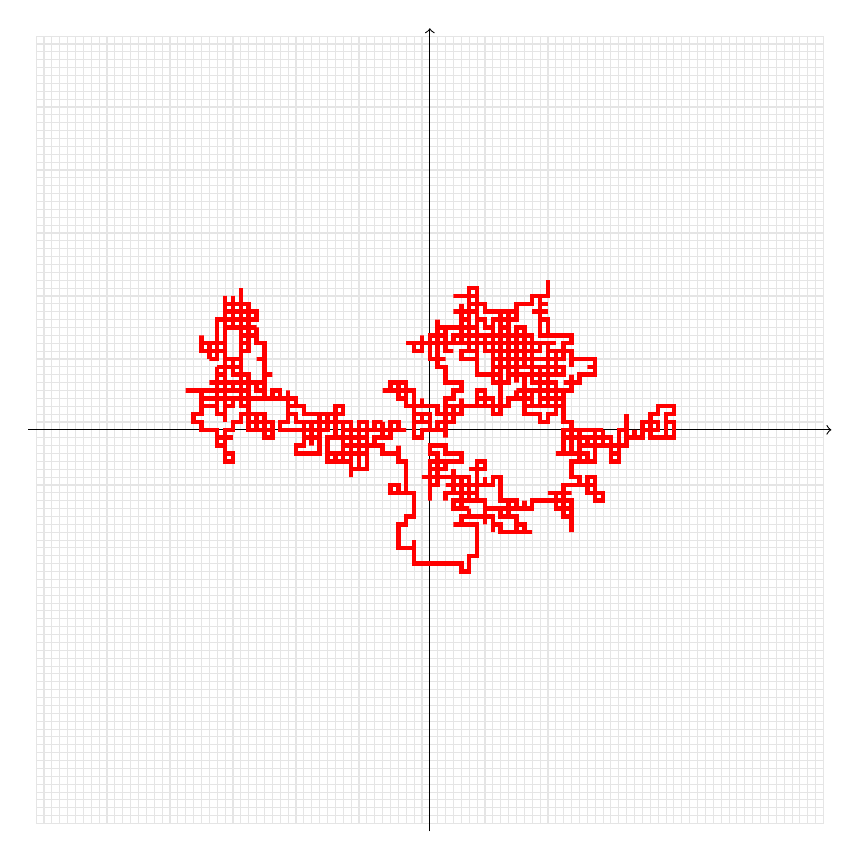
\begin{tikzpicture}[scale = .1]
\draw [black!10] (-50,-50) grid (50,50);
\draw [->] (-51,0) -- (51,0);
\draw [->] (0,-51) -- (0,51);
\draw [ultra thick, red] (0,0) -- ++(1, 0) -- ++(1, 0) -- ++(0, 1) -- ++(1, 0) -- ++(0, 1) -- ++(-1, 0) -- ++(0, -1) -- ++(-1, 0) -- ++(0, -1) -- ++(0, 1) -- ++(0, -1) -- ++(1, 0) -- ++(-1, 0) -- ++(-1, 0) -- ++(1, 0) -- ++(-1, 0) -- ++(-1, 0) -- ++(0, -1) -- ++(-1, 0) -- ++(0, 1) -- ++(0, 1) -- ++(0, 1) -- ++(0, 1) -- ++(-1, 0) -- ++(0, 1) -- ++(-1, 0) -- ++(0, 1) -- ++(0, -1) -- ++(1, 0) -- ++(0, 1) -- ++(-1, 0) -- ++(-1, 0) -- ++(-1, 0) -- ++(1, 0) -- ++(0, 1) -- ++(1, 0) -- ++(1, 0) -- ++(-1, 0) -- ++(0, -1) -- ++(0, 1) -- ++(1, 0) -- ++(0, -1) -- ++(0, -1) -- ++(0, 1) -- ++(0, 1) -- ++(0, -1) -- ++(1, 0) -- ++(0, -1) -- ++(0, 1) -- ++(0, -1) -- ++(0, -1) -- ++(0, -1) -- ++(0, 1) -- ++(0, -1) -- ++(1, 0) -- ++(1, 0) -- ++(0, -1) -- ++(0, -1) -- ++(1, 0) -- ++(-1, 0) -- ++(0, 1) -- ++(0, -1) -- ++(0, 1) -- ++(-1, 0) -- ++(0, 1) -- ++(0, -1) -- ++(-1, 0) -- ++(0, 1) -- ++(0, 1) -- ++(1, 0) -- ++(0, 1) -- ++(0, -1) -- ++(1, 0) -- ++(1, 0) -- ++(0, -1) -- ++(1, 0) -- ++(0, 1) -- ++(0, 1) -- ++(1, 0) -- ++(0, 1) -- ++(0, -1) -- ++(0, 1) -- ++(1, 0) -- ++(0, 1) -- ++(-1, 0) -- ++(-1, 0) -- ++(0, 1) -- ++(0, 1) -- ++(-1, 0) -- ++(0, 1) -- ++(-1, 0) -- ++(0, 1) -- ++(0, 1) -- ++(-1, 0) -- ++(0, -1) -- ++(-1, 0) -- ++(0, 1) -- ++(1, 0) -- ++(0, 1) -- ++(0, -1) -- ++(-1, 0) -- ++(0, -1) -- ++(0, 1) -- ++(-1, 0) -- ++(1, 0) -- ++(1, 0) -- ++(1, 0) -- ++(0, -1) -- ++(0, -1) -- ++(0, 1) -- ++(0, 1) -- ++(1, 0) -- ++(1, 0) -- ++(0, -1) -- ++(1, 0) -- ++(-1, 0) -- ++(0, 1) -- ++(0, -1) -- ++(0, 1) -- ++(-1, 0) -- ++(-1, 0) -- ++(0, -1) -- ++(0, -1) -- ++(1, 0) -- ++(1, 0) -- ++(-1, 0) -- ++(0, 1) -- ++(0, 1) -- ++(0, -1) -- ++(0, 1) -- ++(0, 1) -- ++(0, -1) -- ++(1, 0) -- ++(0, 1) -- ++(-1, 0) -- ++(1, 0) -- ++(0, -1) -- ++(-1, 0) -- ++(-1, 0) -- ++(0, -1) -- ++(0, 1) -- ++(1, 0) -- ++(-1, 0) -- ++(-1, 0) -- ++(1, 0) -- ++(1, 0) -- ++(1, 0) -- ++(-1, 0) -- ++(1, 0) -- ++(1, 0) -- ++(-1, 0) -- ++(1, 0) -- ++(-1, 0) -- ++(0, 1) -- ++(-1, 0) -- ++(0, 1) -- ++(1, 0) -- ++(1, 0) -- ++(1, 0) -- ++(-1, 0) -- ++(-1, 0) -- ++(-1, 0) -- ++(1, 0) -- ++(-1, 0) -- ++(0, 1) -- ++(0, -1) -- ++(0, -1) -- ++(0, 1) -- ++(1, 0) -- ++(0, -1) -- ++(-1, 0) -- ++(-1, 0) -- ++(0, -1) -- ++(1, 0) -- ++(1, 0) -- ++(1, 0) -- ++(-1, 0) -- ++(1, 0) -- ++(0, 1) -- ++(1, 0) -- ++(0, 1) -- ++(1, 0) -- ++(0, -1) -- ++(0, -1) -- ++(0, -1) -- ++(1, 0) -- ++(0, -1) -- ++(0, 1) -- ++(0, 1) -- ++(0, 1) -- ++(1, 0) -- ++(-1, 0) -- ++(-1, 0) -- ++(-1, 0) -- ++(0, -1) -- ++(-1, 0) -- ++(1, 0) -- ++(1, 0) -- ++(1, 0) -- ++(1, 0) -- ++(0, -1) -- ++(1, 0) -- ++(0, 1) -- ++(0, -1) -- ++(0, 1) -- ++(-1, 0) -- ++(0, 1) -- ++(1, 0) -- ++(0, 1) -- ++(0, 1) -- ++(1, 0) -- ++(0, 1) -- ++(0, -1) -- ++(0, -1) -- ++(0, -1) -- ++(0, 1) -- ++(0, -1) -- ++(0, -1) -- ++(0, -1) -- ++(1, 0) -- ++(-1, 0) -- ++(1, 0) -- ++(1, 0) -- ++(-1, 0) -- ++(0, -1) -- ++(-1, 0) -- ++(0, -1) -- ++(0, -1) -- ++(-1, 0) -- ++(-1, 0) -- ++(1, 0) -- ++(1, 0) -- ++(-1, 0) -- ++(1, 0) -- ++(-1, 0) -- ++(1, 0) -- ++(0, 1) -- ++(1, 0) -- ++(0, 1) -- ++(0, 1) -- ++(0, -1) -- ++(-1, 0) -- ++(0, 1) -- ++(0, -1) -- ++(-1, 0) -- ++(0, -1) -- ++(1, 0) -- ++(-1, 0) -- ++(0, 1) -- ++(0, -1) -- ++(0, -1) -- ++(0, -1) -- ++(0, 1) -- ++(1, 0) -- ++(0, 1) -- ++(-1, 0) -- ++(0, -1) -- ++(1, 0) -- ++(0, 1) -- ++(1, 0) -- ++(0, 1) -- ++(0, -1) -- ++(0, 1) -- ++(0, 1) -- ++(0, -1) -- ++(-1, 0) -- ++(1, 0) -- ++(0, -1) -- ++(1, 0) -- ++(0, -1) -- ++(-1, 0) -- ++(1, 0) -- ++(-1, 0) -- ++(1, 0) -- ++(1, 0) -- ++(-1, 0) -- ++(-1, 0) -- ++(0, -1) -- ++(-1, 0) -- ++(-1, 0) -- ++(0, 1) -- ++(-1, 0) -- ++(-1, 0) -- ++(0, 1) -- ++(0, 1) -- ++(-1, 0) -- ++(-1, 0) -- ++(0, 1) -- ++(1, 0) -- ++(1, 0) -- ++(0, 1) -- ++(0, 1) -- ++(0, -1) -- ++(-1, 0) -- ++(0, 1) -- ++(0, 1) -- ++(1, 0) -- ++(-1, 0) -- ++(-1, 0) -- ++(0, 1) -- ++(0, -1) -- ++(-1, 0) -- ++(1, 0) -- ++(1, 0) -- ++(0, 1) -- ++(0, 1) -- ++(0, 1) -- ++(0, 1) -- ++(0, -1) -- ++(0, -1) -- ++(-1, 0) -- ++(-1, 0) -- ++(1, 0) -- ++(0, 1) -- ++(0, -1) -- ++(0, -1) -- ++(1, 0) -- ++(0, 1) -- ++(1, 0) -- ++(0, -1) -- ++(1, 0) -- ++(0, -1) -- ++(1, 0) -- ++(0, -1) -- ++(1, 0) -- ++(1, 0) -- ++(0, -1) -- ++(1, 0) -- ++(0, -1) -- ++(-1, 0) -- ++(0, 1) -- ++(0, -1) -- ++(0, -1) -- ++(0, 1) -- ++(-1, 0) -- ++(0, -1) -- ++(1, 0) -- ++(0, 1) -- ++(1, 0) -- ++(1, 0) -- ++(0, -1) -- ++(0, -1) -- ++(-1, 0) -- ++(0, -1) -- ++(0, 1) -- ++(-1, 0) -- ++(0, 1) -- ++(1, 0) -- ++(0, -1) -- ++(0, -1) -- ++(0, -1) -- ++(0, 1) -- ++(-1, 0) -- ++(1, 0) -- ++(0, 1) -- ++(0, 1) -- ++(1, 0) -- ++(0, 1) -- ++(1, 0) -- ++(0, -1) -- ++(-1, 0) -- ++(-1, 0) -- ++(0, -1) -- ++(1, 0) -- ++(1, 0) -- ++(-1, 0) -- ++(1, 0) -- ++(0, -1) -- ++(0, -1) -- ++(1, 0) -- ++(1, 0) -- ++(-1, 0) -- ++(1, 0) -- ++(-1, 0) -- ++(-1, 0) -- ++(0, 1) -- ++(0, -1) -- ++(0, 1) -- ++(-1, 0) -- ++(-1, 0) -- ++(0, 1) -- ++(-1, 0) -- ++(1, 0) -- ++(0, -1) -- ++(0, 1) -- ++(1, 0) -- ++(0, 1) -- ++(0, 1) -- ++(1, 0) -- ++(0, 1) -- ++(0, 1) -- ++(0, -1) -- ++(1, 0) -- ++(1, 0) -- ++(0, -1) -- ++(0, 1) -- ++(1, 0) -- ++(-1, 0) -- ++(0, -1) -- ++(0, -1) -- ++(1, 0) -- ++(0, 1) -- ++(-1, 0) -- ++(0, -1) -- ++(1, 0) -- ++(-1, 0) -- ++(0, 1) -- ++(1, 0) -- ++(-1, 0) -- ++(0, -1) -- ++(-1, 0) -- ++(-1, 0) -- ++(0, -1) -- ++(0, 1) -- ++(1, 0) -- ++(1, 0) -- ++(0, -1) -- ++(0, 1) -- ++(0, -1) -- ++(0, -1) -- ++(-1, 0) -- ++(0, 1) -- ++(0, -1) -- ++(1, 0) -- ++(-1, 0) -- ++(0, -1) -- ++(-1, 0) -- ++(0, 1) -- ++(0, 1) -- ++(1, 0) -- ++(0, -1) -- ++(1, 0) -- ++(0, -1) -- ++(1, 0) -- ++(0, -1) -- ++(0, 1) -- ++(-1, 0) -- ++(-1, 0) -- ++(0, 1) -- ++(1, 0) -- ++(-1, 0) -- ++(-1, 0) -- ++(0, 1) -- ++(-1, 0) -- ++(-1, 0) -- ++(-1, 0) -- ++(0, -1) -- ++(1, 0) -- ++(1, 0) -- ++(0, -1) -- ++(0, -1) -- ++(-1, 0) -- ++(1, 0) -- ++(1, 0) -- ++(0, -1) -- ++(0, -1) -- ++(1, 0) -- ++(0, 1) -- ++(1, 0) -- ++(0, 1) -- ++(1, 0) -- ++(1, 0) -- ++(1, 0) -- ++(0, 1) -- ++(0, 1) -- ++(0, -1) -- ++(-1, 0) -- ++(1, 0) -- ++(1, 0) -- ++(0, 1) -- ++(1, 0) -- ++(1, 0) -- ++(0, 1) -- ++(-1, 0) -- ++(1, 0) -- ++(0, 1) -- ++(-1, 0) -- ++(1, 0) -- ++(-1, 0) -- ++(1, 0) -- ++(-1, 0) -- ++(-1, 0) -- ++(-1, 0) -- ++(0, -1) -- ++(0, 1) -- ++(0, 1) -- ++(-1, 0) -- ++(0, -1) -- ++(-1, 0) -- ++(0, -1) -- ++(-1, 0) -- ++(-1, 0) -- ++(1, 0) -- ++(1, 0) -- ++(0, -1) -- ++(-1, 0) -- ++(-1, 0) -- ++(0, -1) -- ++(1, 0) -- ++(1, 0) -- ++(-1, 0) -- ++(0, 1) -- ++(1, 0) -- ++(1, 0) -- ++(0, 1) -- ++(-1, 0) -- ++(0, 1) -- ++(0, 1) -- ++(1, 0) -- ++(0, 1) -- ++(1, 0) -- ++(0, 1) -- ++(-1, 0) -- ++(-1, 0) -- ++(-1, 0) -- ++(-1, 0) -- ++(0, 1) -- ++(0, 1) -- ++(1, 0) -- ++(0, -1) -- ++(0, -1) -- ++(-1, 0) -- ++(0, 1) -- ++(0, 1) -- ++(1, 0) -- ++(-1, 0) -- ++(0, 1) -- ++(-1, 0) -- ++(1, 0) -- ++(-1, 0) -- ++(1, 0) -- ++(1, 0) -- ++(-1, 0) -- ++(0, 1) -- ++(0, 1) -- ++(0, -1) -- ++(1, 0) -- ++(-1, 0) -- ++(0, 1) -- ++(1, 0) -- ++(0, 1) -- ++(0, 1) -- ++(0, -1) -- ++(0, -1) -- ++(-1, 0) -- ++(-1, 0) -- ++(0, -1) -- ++(-1, 0) -- ++(-1, 0) -- ++(0, -1) -- ++(-1, 0) -- ++(0, -1) -- ++(0, -1) -- ++(-1, 0) -- ++(1, 0) -- ++(0, -1) -- ++(0, 1) -- ++(0, 1) -- ++(-1, 0) -- ++(1, 0) -- ++(0, -1) -- ++(-1, 0) -- ++(0, -1) -- ++(0, 1) -- ++(0, -1) -- ++(0, -1) -- ++(-1, 0) -- ++(0, 1) -- ++(-1, 0) -- ++(0, -1) -- ++(-1, 0) -- ++(-1, 0) -- ++(0, 1) -- ++(-1, 0) -- ++(1, 0) -- ++(1, 0) -- ++(0, -1) -- ++(-1, 0) -- ++(1, 0) -- ++(0, 1) -- ++(0, 1) -- ++(0, 1) -- ++(0, 1) -- ++(-1, 0) -- ++(1, 0) -- ++(0, 1) -- ++(1, 0) -- ++(-1, 0) -- ++(-1, 0) -- ++(0, 1) -- ++(-1, 0) -- ++(-1, 0) -- ++(1, 0) -- ++(1, 0) -- ++(1, 0) -- ++(-1, 0) -- ++(-1, 0) -- ++(1, 0) -- ++(0, -1) -- ++(0, 1) -- ++(0, 1) -- ++(1, 0) -- ++(-1, 0) -- ++(1, 0) -- ++(0, -1) -- ++(0, -1) -- ++(0, -1) -- ++(0, 1) -- ++(1, 0) -- ++(0, -1) -- ++(1, 0) -- ++(1, 0) -- ++(1, 0) -- ++(1, 0) -- ++(0, -1) -- ++(-1, 0) -- ++(0, -1) -- ++(0, -1) -- ++(0, -1) -- ++(1, 0) -- ++(0, 1) -- ++(0, -1) -- ++(1, 0) -- ++(-1, 0) -- ++(0, 1) -- ++(1, 0) -- ++(0, 1) -- ++(-1, 0) -- ++(0, -1) -- ++(-1, 0) -- ++(0, -1) -- ++(1, 0) -- ++(0, 1) -- ++(0, -1) -- ++(1, 0) -- ++(0, -1) -- ++(1, 0) -- ++(1, 0) -- ++(-1, 0) -- ++(0, 1) -- ++(0, -1) -- ++(1, 0) -- ++(0, 1) -- ++(1, 0) -- ++(-1, 0) -- ++(1, 0) -- ++(0, -1) -- ++(1, 0) -- ++(-1, 0) -- ++(0, 1) -- ++(1, 0) -- ++(-1, 0) -- ++(-1, 0) -- ++(-1, 0) -- ++(-1, 0) -- ++(-1, 0) -- ++(0, 1) -- ++(0, -1) -- ++(0, -1) -- ++(0, -1) -- ++(0, 1) -- ++(0, -1) -- ++(0, 1) -- ++(0, 1) -- ++(0, -1) -- ++(0, 1) -- ++(0, -1) -- ++(0, 1) -- ++(0, 1) -- ++(1, 0) -- ++(-1, 0) -- ++(-1, 0) -- ++(0, -1) -- ++(1, 0) -- ++(-1, 0) -- ++(0, -1) -- ++(0, 1) -- ++(0, 1) -- ++(1, 0) -- ++(-1, 0) -- ++(0, 1) -- ++(0, 1) -- ++(-1, 0) -- ++(0, -1) -- ++(0, 1) -- ++(0, -1) -- ++(0, -1) -- ++(0, -1) -- ++(1, 0) -- ++(1, 0) -- ++(1, 0) -- ++(0, 1) -- ++(1, 0) -- ++(0, -1) -- ++(0, -1) -- ++(-1, 0) -- ++(-1, 0) -- ++(-1, 0) -- ++(0, -1) -- ++(-1, 0) -- ++(-1, 0) -- ++(0, 1) -- ++(1, 0) -- ++(1, 0) -- ++(0, -1) -- ++(-1, 0) -- ++(0, 1) -- ++(0, 1) -- ++(0, -1) -- ++(1, 0) -- ++(-1, 0) -- ++(0, -1) -- ++(0, -1) -- ++(0, -1) -- ++(0, -1) -- ++(0, 1) -- ++(0, -1) -- ++(0, -1) -- ++(0, -1) -- ++(0, -1) -- ++(-1, 0) -- ++(-1, 0) -- ++(1, 0) -- ++(0, 1) -- ++(-1, 0) -- ++(0, -1) -- ++(-1, 0) -- ++(-1, 0) -- ++(-1, 0) -- ++(0, 1) -- ++(0, -1) -- ++(-1, 0) -- ++(0, -1) -- ++(-1, 0) -- ++(0, -1) -- ++(0, -1) -- ++(0, -1) -- ++(0, 1) -- ++(0, 1) -- ++(0, 1) -- ++(0, 1) -- ++(1, 0) -- ++(0, -1) -- ++(-1, 0) -- ++(0, 1) -- ++(0, -1) -- ++(1, 0) -- ++(1, 0) -- ++(0, 1) -- ++(1, 0) -- ++(1, 0) -- ++(0, 1) -- ++(0, 1) -- ++(1, 0) -- ++(0, -1) -- ++(-1, 0) -- ++(0, -1) -- ++(1, 0) -- ++(1, 0) -- ++(1, 0) -- ++(0, -1) -- ++(-1, 0) -- ++(0, 1) -- ++(1, 0) -- ++(-1, 0) -- ++(1, 0) -- ++(1, 0) -- ++(0, 1) -- ++(1, 0) -- ++(0, 1) -- ++(0, -1) -- ++(1, 0) -- ++(0, 1) -- ++(1, 0) -- ++(-1, 0) -- ++(1, 0) -- ++(0, -1) -- ++(0, -1) -- ++(0, 1) -- ++(-1, 0) -- ++(0, -1) -- ++(1, 0) -- ++(-1, 0) -- ++(0, -1) -- ++(1, 0) -- ++(1, 0) -- ++(0, -1) -- ++(0, 1) -- ++(0, -1) -- ++(1, 0) -- ++(0, 1) -- ++(1, 0) -- ++(0, 1) -- ++(0, -1) -- ++(0, 1) -- ++(0, 1) -- ++(0, 1) -- ++(0, 1) -- ++(0, -1) -- ++(0, 1) -- ++(0, -1) -- ++(-1, 0) -- ++(-1, 0) -- ++(0, -1) -- ++(0, 1) -- ++(0, 1) -- ++(0, 1) -- ++(0, -1) -- ++(0, -1) -- ++(-1, 0) -- ++(1, 0) -- ++(1, 0) -- ++(0, 1) -- ++(1, 0) -- ++(0, -1) -- ++(0, -1) -- ++(1, 0) -- ++(0, 1) -- ++(-1, 0) -- ++(-1, 0) -- ++(0, -1) -- ++(0, 1) -- ++(0, -1) -- ++(-1, 0) -- ++(1, 0) -- ++(1, 0) -- ++(-1, 0) -- ++(1, 0) -- ++(-1, 0) -- ++(1, 0) -- ++(-1, 0) -- ++(0, -1) -- ++(-1, 0) -- ++(0, 1) -- ++(1, 0) -- ++(0, -1) -- ++(1, 0) -- ++(1, 0) -- ++(0, 1) -- ++(0, -1) -- ++(0, -1) -- ++(0, -1) -- ++(1, 0) -- ++(0, -1) -- ++(-1, 0) -- ++(0, -1) -- ++(1, 0) -- ++(0, -1) -- ++(0, 1) -- ++(1, 0) -- ++(0, 1) -- ++(0, -1) -- ++(1, 0) -- ++(1, 0) -- ++(1, 0) -- ++(-1, 0) -- ++(-1, 0) -- ++(0, -1) -- ++(1, 0) -- ++(0, -1) -- ++(0, -1) -- ++(-1, 0) -- ++(-1, 0) -- ++(0, 1) -- ++(-1, 0) -- ++(0, 1) -- ++(0, -1) -- ++(1, 0) -- ++(0, 1) -- ++(1, 0) -- ++(1, 0) -- ++(-1, 0) -- ++(-1, 0) -- ++(1, 0) -- ++(1, 0) -- ++(0, -1) -- ++(0, -1) -- ++(0, 1) -- ++(0, 1) -- ++(0, 1) -- ++(0, -1) -- ++(0, 1) -- ++(0, -1) -- ++(1, 0) -- ++(0, 1) -- ++(0, 1) -- ++(0, -1) -- ++(0, -1) -- ++(-1, 0) -- ++(1, 0) -- ++(1, 0) -- ++(0, -1) -- ++(1, 0) -- ++(0, -1) -- ++(-1, 0) -- ++(0, 1) -- ++(1, 0) -- ++(0, 1) -- ++(1, 0) -- ++(0, 1) -- ++(1, 0) -- ++(1, 0) -- ++(0, 1) -- ++(0, 1) -- ++(1, 0) -- ++(0, 1) -- ++(0, -1) -- ++(0, 1) -- ++(1, 0) -- ++(0, 1) -- ++(1, 0) -- ++(1, 0) -- ++(0, -1) -- ++(-1, 0) -- ++(0, -1) -- ++(0, -1) -- ++(0, -1) -- ++(1, 0) -- ++(0, 1) -- ++(0, 1) -- ++(-1, 0) -- ++(0, -1) -- ++(0, -1) -- ++(-1, 0) -- ++(-1, 0) -- ++(0, 1) -- ++(1, 0) -- ++(-1, 0) -- ++(0, 1) -- ++(0, -1) -- ++(1, 0) -- ++(0, 1) -- ++(-1, 0) -- ++(0, -1) -- ++(0, 1) -- ++(0, 1) -- ++(0, -1) -- ++(0, -1) -- ++(-1, 0) -- ++(0, -1) -- ++(-1, 0) -- ++(1, 0) -- ++(-1, 0) -- ++(0, 1) -- ++(0, -1) -- ++(-1, 0) -- ++(0, 1) -- ++(0, 1) -- ++(0, 1) -- ++(0, -1) -- ++(0, -1) -- ++(-1, 0) -- ++(0, -1) -- ++(0, -1) -- ++(-1, 0) -- ++(0, 1) -- ++(-1, 0) -- ++(-1, 0) -- ++(0, 1) -- ++(1, 0) -- ++(-1, 0) -- ++(0, -1) -- ++(0, -1) -- ++(1, 0) -- ++(0, 1) -- ++(-1, 0) -- ++(0, 1) -- ++(-1, 0) -- ++(-1, 0) -- ++(0, -1) -- ++(0, -1) -- ++(0, -1) -- ++(-1, 0) -- ++(-1, 0) -- ++(-1, 0) -- ++(1, 0) -- ++(0, 1) -- ++(0, 1) -- ++(0, 1) -- ++(1, 0) -- ++(-1, 0) -- ++(0, -1) -- ++(1, 0) -- ++(1, 0) -- ++(0, 1) -- ++(-1, 0) -- ++(0, -1) -- ++(1, 0) -- ++(0, -1) -- ++(0, -1) -- ++(1, 0) -- ++(0, -1) -- ++(-1, 0) -- ++(-1, 0) -- ++(0, -1) -- ++(0, -1) -- ++(1, 0) -- ++(0, -1) -- ++(1, 0) -- ++(0, -1) -- ++(1, 0) -- ++(-1, 0) -- ++(1, 0) -- ++(0, -1) -- ++(0, 1) -- ++(-1, 0) -- ++(1, 0) -- ++(0, 1) -- ++(0, 1) -- ++(-1, 0) -- ++(0, -1) -- ++(0, 1) -- ++(0, -1) -- ++(0, -1) -- ++(1, 0) -- ++(1, 0) -- ++(0, -1) -- ++(-1, 0) -- ++(0, 1) -- ++(0, 1) -- ++(-1, 0) -- ++(0, 1) -- ++(0, -1) -- ++(-1, 0) -- ++(-1, 0) -- ++(-1, 0) -- ++(0, -1) -- ++(0, 1) -- ++(0, -1) -- ++(1, 0) -- ++(-1, 0) -- ++(0, -1) -- ++(-1, 0) -- ++(0, -1) -- ++(1, 0) -- ++(0, -1) -- ++(0, 1) -- ++(0, -1) -- ++(0, 1) -- ++(0, 1) -- ++(-1, 0) -- ++(1, 0) -- ++(1, 0) -- ++(0, -1) -- ++(0, -1) -- ++(0, -1) -- ++(0, -1) -- ++(0, 1) -- ++(0, 1) -- ++(0, 1) -- ++(0, -1) -- ++(-1, 0) -- ++(1, 0) -- ++(-1, 0) -- ++(0, 1) -- ++(1, 0) -- ++(0, 1) -- ++(-1, 0) -- ++(0, 1) -- ++(-1, 0) -- ++(-1, 0) -- ++(1, 0) -- ++(0, -1) -- ++(-1, 0) -- ++(-1, 0) -- ++(-1, 0) -- ++(0, -1) -- ++(-1, 0) -- ++(-1, 0) -- ++(-1, 0) -- ++(0, -1) -- ++(-1, 0) -- ++(0, 1) -- ++(-1, 0) -- ++(1, 0) -- ++(-1, 0) -- ++(-1, 0) -- ++(0, 1) -- ++(-1, 0) -- ++(1, 0) -- ++(-1, 0) -- ++(0, 1) -- ++(0, 1) -- ++(0, -1) -- ++(-1, 0) -- ++(0, -1) -- ++(0, 1) -- ++(0, -1) -- ++(1, 0) -- ++(0, 1) -- ++(0, -1) -- ++(0, 1) -- ++(-1, 0) -- ++(-1, 0) -- ++(-1, 0) -- ++(-1, 0) -- ++(0, -1) -- ++(0, 1) -- ++(1, 0) -- ++(1, 0) -- ++(0, 1) -- ++(1, 0) -- ++(-1, 0) -- ++(-1, 0) -- ++(1, 0) -- ++(0, 1) -- ++(-1, 0) -- ++(0, 1) -- ++(0, -1) -- ++(0, -1) -- ++(0, 1) -- ++(0, -1) -- ++(1, 0) -- ++(-1, 0) -- ++(1, 0) -- ++(1, 0) -- ++(0, -1) -- ++(-1, 0) -- ++(-1, 0) -- ++(0, 1) -- ++(-1, 0) -- ++(1, 0) -- ++(0, 1) -- ++(-1, 0) -- ++(-1, 0) -- ++(0, -1) -- ++(-1, 0) -- ++(0, -1) -- ++(0, -1) -- ++(0, 1) -- ++(0, 1) -- ++(0, 1) -- ++(-1, 0) -- ++(1, 0) -- ++(1, 0) -- ++(-1, 0) -- ++(0, 1) -- ++(1, 0) -- ++(0, 1) -- ++(0, -1) -- ++(1, 0) -- ++(-1, 0) -- ++(0, 1) -- ++(0, -1) -- ++(-1, 0) -- ++(0, 1) -- ++(0, -1) -- ++(0, 1) -- ++(1, 0) -- ++(0, 1) -- ++(-1, 0) -- ++(0, 1) -- ++(1, 0) -- ++(1, 0) -- ++(0, -1) -- ++(1, 0) -- ++(1, 0) -- ++(0, -1) -- ++(-1, 0) -- ++(-1, 0) -- ++(-1, 0) -- ++(0, -1) -- ++(0, 1) -- ++(1, 0) -- ++(0, -1) -- ++(-1, 0) -- ++(0, 1) -- ++(0, -1) -- ++(0, -1) -- ++(1, 0) -- ++(1, 0) -- ++(1, 0) -- ++(1, 0) -- ++(0, -1) -- ++(0, 1) -- ++(0, -1) -- ++(-1, 0) -- ++(0, -1) -- ++(0, -1) -- ++(0, -1) -- ++(1, 0) -- ++(-1, 0) -- ++(0, 1) -- ++(-1, 0) -- ++(1, 0) -- ++(0, -1) -- ++(-1, 0) -- ++(0, 1) -- ++(1, 0) -- ++(0, 1) -- ++(-1, 0) -- ++(1, 0) -- ++(1, 0) -- ++(-1, 0) -- ++(0, -1) -- ++(1, 0) -- ++(0, 1) -- ++(0, 1) -- ++(0, 1) -- ++(0, -1) -- ++(1, 0) -- ++(-1, 0) -- ++(1, 0) -- ++(0, 1) -- ++(0, 1) -- ++(0, 1) -- ++(1, 0) -- ++(0, -1) -- ++(-1, 0) -- ++(-1, 0) -- ++(1, 0) -- ++(0, -1) -- ++(0, -1) -- ++(1, 0) -- ++(0, 1) -- ++(0, -1) -- ++(1, 0) -- ++(0, 1) -- ++(1, 0) -- ++(0, -1) -- ++(0, -1) -- ++(0, -1) -- ++(1, 0) -- ++(-1, 0) -- ++(1, 0) -- ++(0, -1) -- ++(0, -1) -- ++(-1, 0) -- ++(0, 1) -- ++(1, 0) -- ++(0, 1) -- ++(-1, 0) -- ++(1, 0) -- ++(1, 0) -- ++(0, -1) -- ++(1, 0) -- ++(0, 1) -- ++(0, -1) -- ++(-1, 0) -- ++(-1, 0) -- ++(0, -1) -- ++(1, 0) -- ++(-1, 0) -- ++(1, 0) -- ++(0, -1) -- ++(1, 0) -- ++(0, -1) -- ++(1, 0) -- ++(-1, 0) -- ++(-1, 0) -- ++(0, 1) -- ++(0, -1) -- ++(-1, 0) -- ++(-1, 0) -- ++(0, 1) -- ++(-1, 0) -- ++(0, -1) -- ++(0, 1) -- ++(0, 1) -- ++(0, -1) -- ++(0, 1) -- ++(-1, 0) -- ++(-1, 0) -- ++(1, 0) -- ++(0, 1) -- ++(0, -1) -- ++(0, -1) -- ++(0, 1) -- ++(-1, 0) -- ++(-1, 0) -- ++(0, 1) -- ++(0, -1) -- ++(-1, 0) -- ++(0, -1) -- ++(-1, 0) -- ++(1, 0) -- ++(1, 0) -- ++(-1, 0) -- ++(1, 0) -- ++(1, 0) -- ++(0, -1) -- ++(0, -1) -- ++(0, -1) -- ++(0, -1) -- ++(-1, 0) -- ++(0, -1) -- ++(0, -1) -- ++(-1, 0) -- ++(0, 1) -- ++(-1, 0) -- ++(1, 0) -- ++(-1, 0) -- ++(-1, 0) -- ++(-1, 0) -- ++(-1, 0) -- ++(-1, 0) -- ++(-1, 0) -- ++(1, 0) -- ++(-1, 0) -- ++(0, 1) -- ++(0, 1) -- ++(0, 1) -- ++(0, -1) -- ++(-1, 0) -- ++(-1, 0) -- ++(0, 1) -- ++(0, 1) -- ++(0, 1) -- ++(0, -1) -- ++(0, 1) -- ++(1, 0) -- ++(0, 1) -- ++(1, 0) -- ++(0, 1) -- ++(0, 1) -- ++(0, 1) -- ++(-1, 0) -- ++(-1, 0) -- ++(-1, 0) -- ++(0, 1) -- ++(1, 0) -- ++(-1, 0) -- ++(1, 0) -- ++(0, -1) -- ++(1, 0) -- ++(0, 1) -- ++(0, 1) -- ++(0, 1) -- ++(0, 1) -- ++(-1, 0) -- ++(0, 1) -- ++(0, 1) -- ++(0, -1) -- ++(0, 1) -- ++(0, -1) -- ++(-1, 0) -- ++(-1, 0) -- ++(1, 0) -- ++(-1, 0) -- ++(0, 1) -- ++(-1, 0) -- ++(-1, 0) -- ++(0, 1) -- ++(0, 1) -- ++(1, 0) -- ++(1, 0) -- ++(1, 0) -- ++(0, -1) -- ++(0, 1) -- ++(0, 1) -- ++(1, 0) -- ++(-1, 0) -- ++(0, -1) -- ++(0, 1) -- ++(0, -1) -- ++(0, -1) -- ++(-1, 0) -- ++(0, 1) -- ++(1, 0) -- ++(1, 0) -- ++(1, 0) -- ++(-1, 0) -- ++(-1, 0) -- ++(1, 0) -- ++(-1, 0) -- ++(1, 0) -- ++(0, 1) -- ++(-1, 0) -- ++(0, -1) -- ++(-1, 0) -- ++(-1, 0) -- ++(0, 1) -- ++(1, 0) -- ++(-1, 0) -- ++(0, -1) -- ++(1, 0) -- ++(0, 1) -- ++(0, -1) -- ++(-1, 0) -- ++(1, 0) -- ++(1, 0) -- ++(0, -1) -- ++(0, 1) -- ++(0, -1) -- ++(0, 1) -- ++(-1, 0) -- ++(0, -1) -- ++(-1, 0) -- ++(0, -1) -- ++(-1, 0) -- ++(-1, 0) -- ++(1, 0) -- ++(0, -1) -- ++(0, 1) -- ++(0, -1) -- ++(0, 1) -- ++(-1, 0) -- ++(-1, 0) -- ++(0, -1) -- ++(1, 0) -- ++(-1, 0) -- ++(0, -1) -- ++(-1, 0) -- ++(0, 1) -- ++(0, -1) -- ++(1, 0) -- ++(0, -1) -- ++(0, -1) -- ++(0, 1) -- ++(0, 1) -- ++(0, 1) -- ++(-1, 0) -- ++(1, 0) -- ++(1, 0) -- ++(-1, 0) -- ++(-1, 0) -- ++(0, 1) -- ++(0, 1) -- ++(1, 0) -- ++(1, 0) -- ++(0, -1) -- ++(0, 1) -- ++(0, 1) -- ++(1, 0) -- ++(0, 1) -- ++(-1, 0) -- ++(0, -1) -- ++(-1, 0) -- ++(0, -1) -- ++(1, 0) -- ++(-1, 0) -- ++(0, 1) -- ++(-1, 0) -- ++(1, 0) -- ++(1, 0) -- ++(0, -1) -- ++(-1, 0) -- ++(0, -1) -- ++(-1, 0) -- ++(0, -1) -- ++(-1, 0) -- ++(1, 0) -- ++(1, 0) -- ++(0, 1) -- ++(0, 1) -- ++(0, 1) -- ++(0, 1) -- ++(0, -1) -- ++(0, 1) -- ++(-1, 0) -- ++(0, -1) -- ++(1, 0) -- ++(-1, 0) -- ++(0, -1) -- ++(-1, 0) -- ++(0, 1) -- ++(0, -1) -- ++(-1, 0) -- ++(0, -1) -- ++(0, -1) -- ++(1, 0) -- ++(0, -1) -- ++(-1, 0) -- ++(0, 1) -- ++(1, 0) -- ++(-1, 0) -- ++(0, -1) -- ++(1, 0) -- ++(1, 0) -- ++(0, 1) -- ++(0, 1) -- ++(1, 0) -- ++(1, 0) -- ++(-1, 0) -- ++(1, 0) -- ++(0, -1) -- ++(1, 0) -- ++(0, -1) -- ++(0, -1) -- ++(-1, 0) -- ++(-1, 0) -- ++(1, 0) -- ++(0, 1) -- ++(0, 1) -- ++(0, 1) -- ++(1, 0) -- ++(1, 0) -- ++(-1, 0) -- ++(0, 1) -- ++(-1, 0) -- ++(-1, 0) -- ++(0, -1) -- ++(-1, 0) -- ++(0, 1) -- ++(0, 1) -- ++(0, -1) -- ++(0, 1) -- ++(0, -1) -- ++(-1, 0) -- ++(1, 0) -- ++(0, 1) -- ++(0, 1) -- ++(-1, 0) -- ++(-1, 0) -- ++(0, 1) -- ++(-1, 0) -- ++(0, -1) -- ++(0, -1) -- ++(0, -1) -- ++(-1, 0) -- ++(0, -1) -- ++(0, 1) -- ++(-1, 0) -- ++(0, 1) -- ++(-1, 0) -- ++(-1, 0) -- ++(-1, 0) -- ++(0, 1) -- ++(1, 0) -- ++(0, 1) -- ++(0, 1) -- ++(0, 1) -- ++(1, 0) -- ++(0, -1) -- ++(-1, 0) -- ++(0, -1) -- ++(1, 0) -- ++(0, -1) -- ++(1, 0) -- ++(1, 0) -- ++(0, -1) -- ++(-1, 0) -- ++(1, 0) -- ++(1, 0) -- ++(-1, 0) -- ++(1, 0) -- ++(1, 0) -- ++(0, 1) -- ++(1, 0) -- ++(0, 1) -- ++(1, 0) -- ++(0, 1) -- ++(-1, 0) -- ++(0, -1) -- ++(-1, 0) -- ++(0, -1) -- ++(0, 1) -- ++(0, -1) -- ++(0, -1) -- ++(-1, 0) -- ++(0, -1) -- ++(0, -1) -- ++(0, -1) -- ++(0, 1) -- ++(0, -1) -- ++(-1, 0) -- ++(-1, 0) -- ++(1, 0) -- ++(-1, 0) -- ++(-1, 0) -- ++(0, 1) -- ++(1, 0) -- ++(0, 1) -- ++(0, 1) -- ++(-1, 0) -- ++(-1, 0) -- ++(1, 0) -- ++(1, 0) -- ++(1, 0) -- ++(0, -1) -- ++(0, -1) -- ++(0, 1) -- ++(0, 1) -- ++(0, 1) -- ++(-1, 0) -- ++(0, -1) -- ++(1, 0) -- ++(0, 1) -- ++(1, 0) -- ++(1, 0) -- ++(1, 0) -- ++(0, -1) -- ++(0, 1) -- ++(-1, 0) -- ++(0, 1) -- ++(-1, 0) -- ++(-1, 0) -- ++(1, 0) -- ++(-1, 0) -- ++(-1, 0) -- ++(0, 1) -- ++(-1, 0) -- ++(0, 1) -- ++(-1, 0) -- ++(1, 0) -- ++(-1, 0) -- ++(0, 1) -- ++(0, -1) -- ++(-1, 0) -- ++(0, 1) -- ++(-1, 0) -- ++(0, -1) -- ++(1, 0) -- ++(-1, 0) -- ++(0, 1) -- ++(0, -1) -- ++(-1, 0) -- ++(0, 1) -- ++(0, 1) -- ++(-1, 0) -- ++(0, -1) -- ++(1, 0) -- ++(0, 1) -- ++(0, -1) -- ++(0, 1) -- ++(0, -1) -- ++(-1, 0) -- ++(0, 1) -- ++(-1, 0) -- ++(-1, 0) -- ++(0, -1) -- ++(0, 1) -- ++(0, -1) -- ++(0, 1) -- ++(0, 1) -- ++(0, 1) -- ++(0, 1) -- ++(0, 1) -- ++(1, 0) -- ++(0, 1) -- ++(-1, 0) -- ++(0, 1) -- ++(0, -1) -- ++(0, -1) -- ++(1, 0) -- ++(0, 1) -- ++(-1, 0) -- ++(1, 0) -- ++(0, 1) -- ++(1, 0) -- ++(-1, 0) -- ++(1, 0) -- ++(0, 1) -- ++(0, -1) -- ++(0, -1) -- ++(1, 0) -- ++(0, -1) -- ++(0, -1) -- ++(0, -1) -- ++(0, 1) -- ++(-1, 0) -- ++(1, 0) -- ++(0, -1) -- ++(0, -1) -- ++(1, 0) -- ++(-1, 0) -- ++(0, -1) -- ++(0, -1) -- ++(-1, 0) -- ++(0, 1) -- ++(-1, 0) -- ++(0, 1) -- ++(-1, 0) -- ++(0, -1) -- ++(-1, 0) -- ++(0, -1) -- ++(1, 0) -- ++(0, 1) -- ++(0, 1) -- ++(0, -1) -- ++(0, 1) -- ++(-1, 0) -- ++(0, 1) -- ++(1, 0) -- ++(0, 1) -- ++(-1, 0) -- ++(-1, 0) -- ++(0, -1) -- ++(-1, 0) -- ++(1, 0) -- ++(0, 1) -- ++(0, 1) -- ++(0, 1) -- ++(-1, 0) -- ++(-1, 0) -- ++(1, 0) -- ++(1, 0) -- ++(0, 1) -- ++(0, 1) -- ++(1, 0) -- ++(0, 1) -- ++(0, -1) -- ++(0, 1) -- ++(1, 0) -- ++(0, 1) -- ++(1, 0) -- ++(0, -1) -- ++(0, -1) -- ++(0, 1) -- ++(-1, 0) -- ++(0, -1) -- ++(1, 0) -- ++(0, 1) -- ++(-1, 0) -- ++(0, 1) -- ++(0, 1) -- ++(0, 1) -- ++(0, 1) -- ++(0, -1) -- ++(0, -1) -- ++(0, -1) -- ++(0, -1) -- ++(0, -1) -- ++(-1, 0) -- ++(0, 1) -- ++(0, 1) -- ++(1, 0) -- ++(1, 0) -- ++(0, 1) -- ++(0, -1) -- ++(1, 0) -- ++(-1, 0) -- ++(0, 1) -- ++(-1, 0) -- ++(-1, 0) -- ++(0, -1) -- ++(-1, 0) -- ++(0, 1) -- ++(1, 0) -- ++(-1, 0) -- ++(0, -1) -- ++(1, 0) -- ++(0, 1) -- ++(0, -1) -- ++(0, 1) -- ++(0, -1) -- ++(0, 1) -- ++(1, 0) -- ++(-1, 0) -- ++(1, 0) -- ++(1, 0) -- ++(0, -1) -- ++(-1, 0) -- ++(1, 0) -- ++(0, 1) -- ++(-1, 0) -- ++(0, 1) -- ++(0, 1) -- ++(0, -1) -- ++(0, -1) -- ++(-1, 0) -- ++(0, 1) -- ++(0, -1) -- ++(-1, 0) -- ++(0, 1) -- ++(0, -1) -- ++(0, -1) -- ++(0, 1) -- ++(1, 0) -- ++(-1, 0) -- ++(0, -1) -- ++(0, 1) -- ++(0, -1) -- ++(1, 0) -- ++(-1, 0) -- ++(0, -1) -- ++(0, 1) -- ++(1, 0) -- ++(0, 1) -- ++(1, 0) -- ++(0, -1) -- ++(1, 0) -- ++(1, 0) -- ++(0, -1) -- ++(-1, 0) -- ++(0, -1) -- ++(1, 0) -- ++(-1, 0) -- ++(0, 1) -- ++(-1, 0) -- ++(1, 0) -- ++(0, -1) -- ++(0, -1) -- ++(-1, 0) -- ++(0, 1) -- ++(-1, 0) -- ++(-1, 0) -- ++(0, 1) -- ++(1, 0) -- ++(0, 1) -- ++(0, -1) -- ++(-1, 0) -- ++(-1, 0) -- ++(0, -1) -- ++(0, -1) -- ++(0, -1) -- ++(0, -1) -- ++(-1, 0) -- ++(-1, 0) -- ++(0, 1) -- ++(0, 1) -- ++(0, -1) -- ++(1, 0) -- ++(0, -1) -- ++(0, -1) -- ++(0, 1) -- ++(1, 0) -- ++(0, -1) -- ++(-1, 0) -- ++(1, 0) -- ++(0, 1) -- ++(1, 0) -- ++(0, -1) -- ++(0, -1) -- ++(0, -1) -- ++(0, -1) -- ++(0, -1) -- ++(1, 0) -- ++(1, 0) -- ++(0, -1) -- ++(0, 1) -- ++(1, 0) -- ++(0, 1) -- ++(-1, 0) -- ++(0, -1) -- ++(0, -1) -- ++(-1, 0) -- ++(1, 0) -- ++(1, 0) -- ++(1, 0) -- ++(-1, 0) -- ++(1, 0) -- ++(1, 0) -- ++(-1, 0) -- ++(-1, 0) -- ++(0, 1) -- ++(0, -1) -- ++(1, 0) -- ++(-1, 0) -- ++(0, -1) -- ++(0, -1) -- ++(1, 0) -- ++(1, 0) -- ++(-1, 0) -- ++(-1, 0) -- ++(1, 0) -- ++(0, -1) -- ++(1, 0) -- ++(1, 0) -- ++(0, -1) -- ++(0, 1) -- ++(0, -1) -- ++(0, -1) -- ++(0, 1) -- ++(-1, 0) -- ++(0, -1) -- ++(1, 0) -- ++(0, 1) -- ++(0, -1) -- ++(0, 1) -- ++(0, -1) -- ++(-1, 0) -- ++(0, 1) -- ++(-1, 0) -- ++(0, 1) -- ++(-1, 0) -- ++(0, -1) -- ++(1, 0) -- ++(1, 0) -- ++(0, 1) -- ++(1, 0) -- ++(-1, 0) -- ++(0, -1) -- ++(1, 0) -- ++(0, 1) -- ++(-1, 0) -- ++(1, 0) -- ++(-1, 0) -- ++(0, 1) -- ++(-1, 0) -- ++(-1, 0) -- ++(0, 1) -- ++(-1, 0) -- ++(0, 1) -- ++(-1, 0) -- ++(1, 0) -- ++(1, 0) -- ++(-1, 0) -- ++(0, 1) -- ++(-1, 0) -- ++(0, 1) -- ++(-1, 0) -- ++(-1, 0) -- ++(-1, 0) -- ++(1, 0) -- ++(-1, 0) -- ++(1, 0) -- ++(0, 1) -- ++(0, 1) -- ++(0, -1) -- ++(1, 0) -- ++(0, -1) -- ++(0, 1) -- ++(0, 1) -- ++(1, 0) -- ++(-1, 0) -- ++(0, 1) -- ++(1, 0) -- ++(0, -1) -- ++(1, 0) -- ++(-1, 0) -- ++(-1, 0) -- ++(0, -1) -- ++(0, -1) -- ++(-1, 0) -- ++(0, 1) -- ++(0, -1) -- ++(0, -1) -- ++(0, -1) -- ++(1, 0) -- ++(-1, 0) -- ++(0, 1) -- ++(-1, 0) -- ++(-1, 0) -- ++(-1, 0) -- ++(-1, 0) -- ++(1, 0) -- ++(1, 0) -- ++(0, -1) -- ++(0, -1) -- ++(1, 0) -- ++(1, 0) -- ++(0, -1) -- ++(1, 0) -- ++(0, 1) -- ++(0, -1) -- ++(0, -1) -- ++(0, 1) -- ++(0, 1) -- ++(1, 0) -- ++(0, 1) -- ++(-1, 0) -- ++(0, -1) -- ++(0, 1) -- ++(0, 1) -- ++(0, 1) -- ++(0, 1) -- ++(0, 1) -- ++(0, -1) -- ++(0, -1) -- ++(0, -1) -- ++(-1, 0) -- ++(0, 1) -- ++(0, -1) -- ++(0, -1) -- ++(-1, 0) -- ++(1, 0) -- ++(0, 1) -- ++(0, -1) -- ++(0, -1) -- ++(0, 1) -- ++(-1, 0) -- ++(-1, 0) -- ++(0, -1) -- ++(0, -1) -- ++(-1, 0) -- ++(0, -1) -- ++(1, 0) -- ++(0, -1) -- ++(1, 0) -- ++(1, 0) -- ++(0, -1) -- ++(1, 0) -- ++(0, -1) -- ++(-1, 0) -- ++(0, 1) -- ++(1, 0) -- ++(1, 0) -- ++(-1, 0) -- ++(0, -1) -- ++(0, -1) -- ++(0, -1) -- ++(1, 0) -- ++(0, 1) -- ++(-1, 0) -- ++(0, 1) -- ++(-1, 0) -- ++(1, 0) -- ++(0, 1) -- ++(-1, 0) -- ++(1, 0) -- ++(0, 1) -- ++(1, 0) -- ++(0, 1) -- ++(1, 0) -- ++(0, 1) -- ++(1, 0) -- ++(0, 1) -- ++(0, -1) -- ++(0, -1);
\end{tikzpicture}
 
\end{center}

\end{document}
